%   Casey O'kane - casey.okane@uky.edu
%   Joe Weisbrod - jtwe226@uky.edu
%   Tristan Cheam - tlcheam01@uky.edu
%   EE480 - Assignment 3: A Faster IDIOT
%   note.tex : Implementor's Note
%   Version:
%       02-14-2016 : initial


\documentclass[conference]{IEEEtran}
\usepackage{graphicx}
\usepackage{float}
\usepackage{verbatim}
\usepackage{adjustbox}

\begin{document}
\title{Assignment 3: A Faster IDIOT\\Implementor's Notes}
\author{\IEEEauthorblockN{Casey O'Kane}
        \IEEEauthorblockA{casey.okane@uky.edu}
        \IEEEauthorblockN{Joe Weisbrod}
        \IEEEauthorblockA{jtwe226@uky.edu}
        \IEEEauthorblockN{Tristan Cheam}
        \IEEEauthorblockA{tlcheam01@uky.edu}}

\maketitle

\begin{abstract}
The goal of this assignment involved implementing the pipelined version of 
the IDIOT instruction set using the AIK assembler, the Verilog Hardware
Design Language and detailed test plan to exhaustively test the different 
components and logic of the design. 
\end{abstract}

\section{General Approach}
Following the approach of previous assignments, the implementation of this 
assignment closely followed a heavily modulated design. Both the data and 
instruction memories where treated as modules along with the ALU incrementor,
ALU module (for ALU instructions), the dependency detection module, the 
register file and the processor itself. 

Similar to the previous assignment, global constants were declared both to 
represent common data structures (like 'WORD) and the different Opcode 
signals that could be received by the processor (like 'OpAdd or any of the 
instructions specified by the IDIOT ISA). Also, the AIK specification IDIOT\_SPEC
provided by Dr. Dietz following the submission of Assignment 2 was used
for the sake of consistency.

The main point of difference for this assignment is the addition of the three
buffer modules that are used to share information between modules of the 
different cycles (Instruction Fetch, Register Read, ALU/Memory, Register
Write). These buffers are used to implement the pipelined design and their 
implementations are described in the next section.

While there are still some incomplete aspects of this assignment (these issues 
are discussed in the \textbf{Issues} section of these notes), the most recent 
diagram is shown in \textbf{Appendix A} at the end of these notes. 

\subsection{Key Notes}
Currently every buffer uses an LI register that interacts with the Dependency
Detector module to implement value forwarding

Also, the ALU uses an additional operation to directly store values into 
memory. This is slightly different than what was suggested during class 
and is detailed in the \textbf{Implementation: Stage 3} section of these 
notes. 
%Other Key Notes here

%%%%%%%%%%%%%%%%%%%%
\section{Implementation}
This section describes how each module was implemented.

\subsection{Dependency Detector}
Module that is used to handle value forwarding/interlock. Basically it checks
the LI register in each of the buffers and enables that buffer (allowing it to 
continue) as long as a dependency issue has not arisen 

\subsection{Stage 0: Instruction Fetch}
\subsubsection{Instruction Memory}
Memory that interacts with the program counter and instruction buffer, the IR assigns
the values of the opcode, destination and source to different values that are sent 
to the instruction register. These instructions are instantiated on reset by the "inst.txt"
file located in the ReqFiles directory.

\subsubsection{Instruction Buffer}
Taking signals from the Instruction memory, the Instruction buffer checks it's NOP
register to determine if a squash/jump has taken place. If so, it sets it's output 
signals to zero. It holds values and sends them to the register file if not squashed.

\subsubsection{Incrementor}
Small module that is used to account for li instructions after a squash by checking 
for an enable signal and incrementing based on input.
 
\subsection{Stage 1: Register Read} 
\subsubsection{Register File}
Used to store information in desired registers, the register file (known as \textbf{registers}
in the source) defines the memory used by processor, assign source and destination addresses,
transfers it's values to the Register Buffer and ensures that that four special purpose 
registers will not be overwritten.

\subsubsection{Register Buffer}
Taking its input signals from the Register File and the Instruction Buffer, the Register
Buffer checks the NOP register like the previous buffer and reacts in the same way
as the Instruction Buffer. 



\subsection{Stage 2: ALU/Memory} 
Important to note here, is that this is primarily where the JZ/SZ/SYZ/FP operations 
are accounted for. After instantiating the three modules below, the \textit{li2ndWord} 
variable is used to determine in the current instruction is the second word of li
instruction. After making this check, the ALU operation is accounted for by checking 
the signal associated with \textit{AluOp} and then setting the squashEnable
or \textit{jumpEnable} if those cases are met, or a sys call if necessary. 

\subsubsection{ALU}
Handled similarly to ALU in some of the team member's Assignment 2 solutions , the 
ALU module takes an opcode and two number inputs, and preforms the operation 
using a case statement and the Verilog compiler.


\subsubsection{Data Memory}
Memory that communicates between the Register Buffer and ALU/Write Buffer, the 
Data Memory sends the ALU/Write Buffer the readAddr signal passed from the
Register Buffer and then writes the result into memory if the right enable received
from the Register Buffer is equal to 1.   

\subsubsection{ALU/Write Buffer}
Again, the ALU/Write buffer is is essentially the same as the previous two buffers 
except that it takes inputs from the Data Memory, ALU and Register Buffer modules.
It checks the buffer's NOP register and then resets values accordingly.

\subsection{Stage 3: Register Write}
 This section is important to note as it is where the load/store operations are implemented.

\subsection{Processor}
Used to instantiate all of the previously defined modules, the processor initializes all 
of the necessary variables that will be used and then calls these modules in succession.

First, Dependency Detection is created after initializing each of the li flags for the buffers, 
and the processor reset is defined. Then the processor looks to account for NOPS and 
li flags before going through each of the pipeline cycles detailed above.


%%%%%%%%%%%%%%%%%%%%%%

\section{Testing}

\subsection{Utilization of GTKWave}
The primary source of testing for this assignment included extensive debugging using the 
GTKWave application after compiling the source using iVerilog. Simple test files were 
written using the ISA instructions formed into assembly using the AIK specification provided by Dr. Dietz (aikspec in the IDIOTSource Directory) and tested using GTKWave. 

\subsection{Included Test Files}
Currently there are two files that were used to test written code:
\subsubsection{test1Src.txt/inst.txt}
This is same example provided by Dr. Dietz in the assignment 3 prompt, it goes through
each of the operations and ensures that it is working correctly. This was used as our main 
test file as it seemed to provide good coverage over the different cases that we hoped to test

\subsubsection{lijmptest.txt/inst1.txt}
This is simple assembly file that was created while debugging the code using GTKwave. It essentially preforms a simple test  that looks at load immediate and jump operations.

\subsection{Test Coverage}

%%%%%%%%%%%%%%%%%%%%%%%
\section{Issues}
\subsection{Features Not implemented}
Currently all instructions in the IDIOT ISA seem to implemented as
designed. Some issues may lie with with limited ability of the provided testbench as 
it primarily consists of two separate test files inst.txt and inst2.txt.  While these two
files are able to test the majority of the necessary instructions used, there are still 

\subsection{Notable workarounds}
\subsubsection{LI Register }
As mentioned in the \textbf{General Approach} section of this report, currently 
every buffer contains a li register that is used to interface the dependency detector
to determine if a buffer should be paused or not. 
\subsubsection{Load/Store}
To account for the Load or Store instructions, the stored opcode \textit{opOut} is 
used to determine if a load or store is occurring and then enable the write enable
value in memory. 

\subsection{Known Errors}
As it currently stands there are no known issues, but this might just involve issues 
created by the limited test files (as detailed above). All aspects of the assignment
seemed to be functional in the debugging process but things might be incorrect due
to 

\subsection{Possible Errors}
While everything appears to be functional there might be some issues with load/store
 operations as they are essentially implemented as a separate opcode for the ALU. 

%%%%%%%%%%%%%%%%%%%%%%%

\section{APPENDIX}
\subsection{Top Level Design}
The high level diagram for the processor is shown on the following page. A larger copy can be found in this directory as well. 

\clearpage

\begin{figure}
\centering
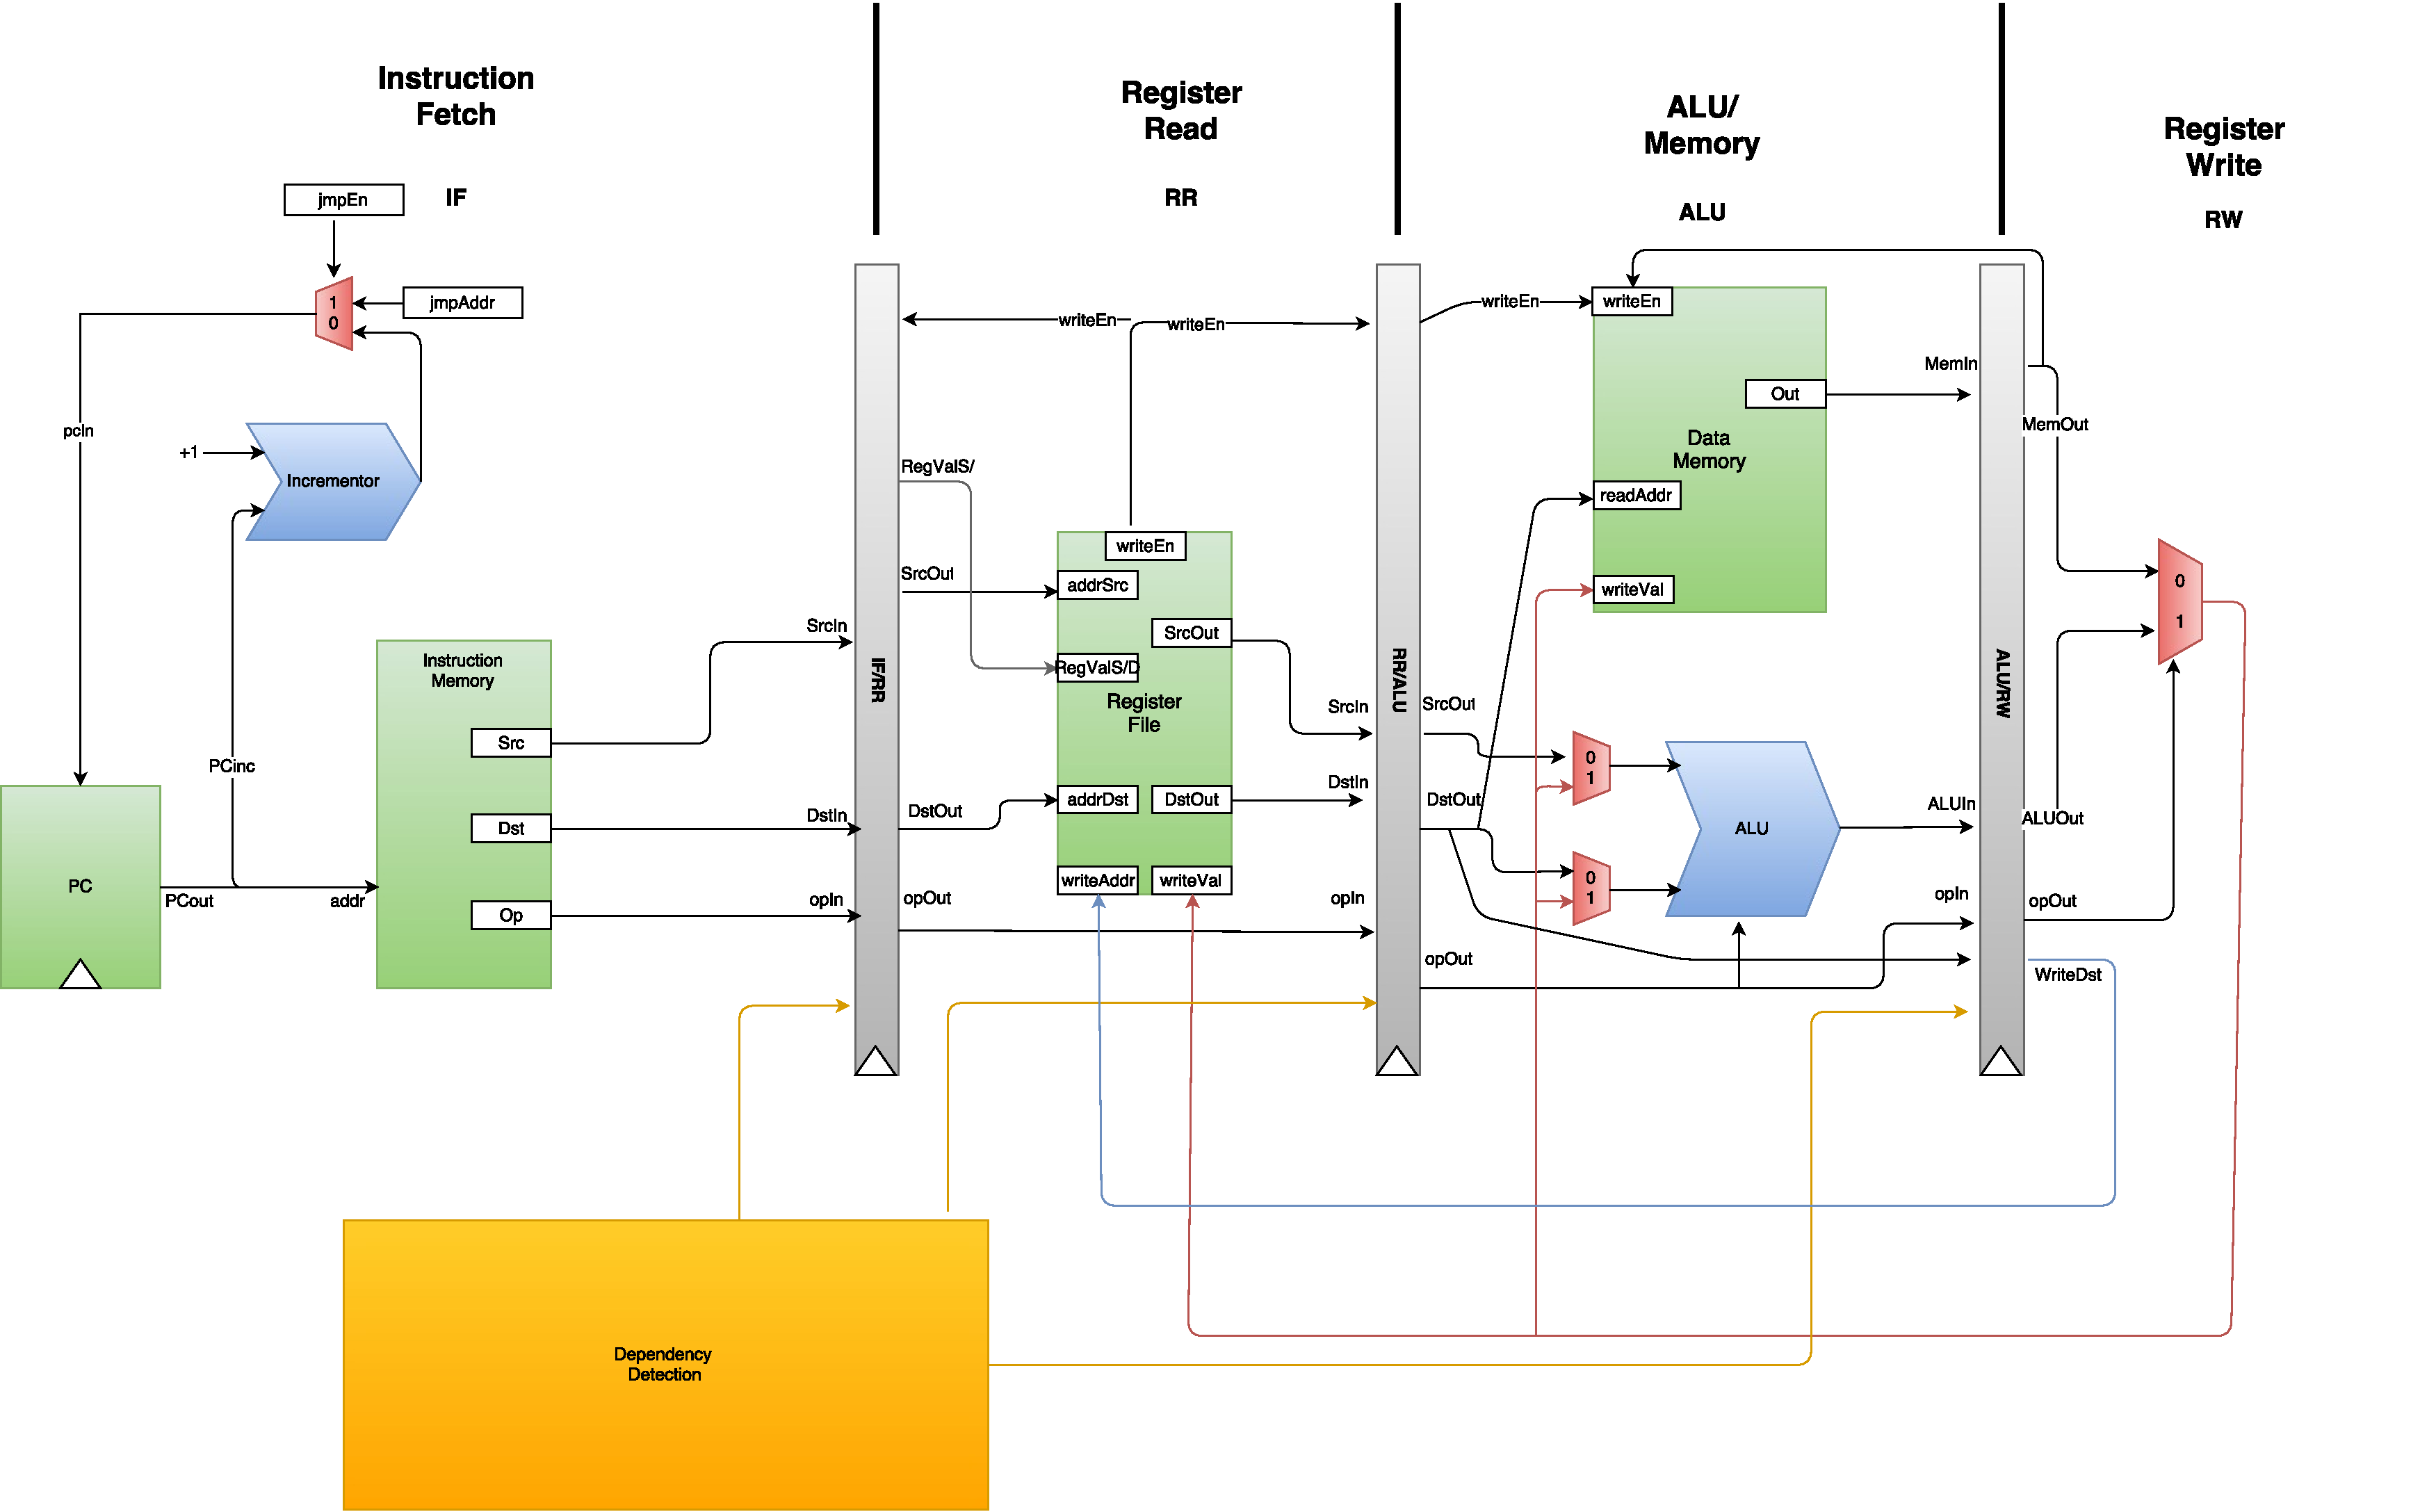
\includegraphics[scale=0.33]{DraftDesign.pdf}
\caption{Initial }
\label{Design Draft}
\end{figure}



\end{document}
